\begin{figure}
  \centerline{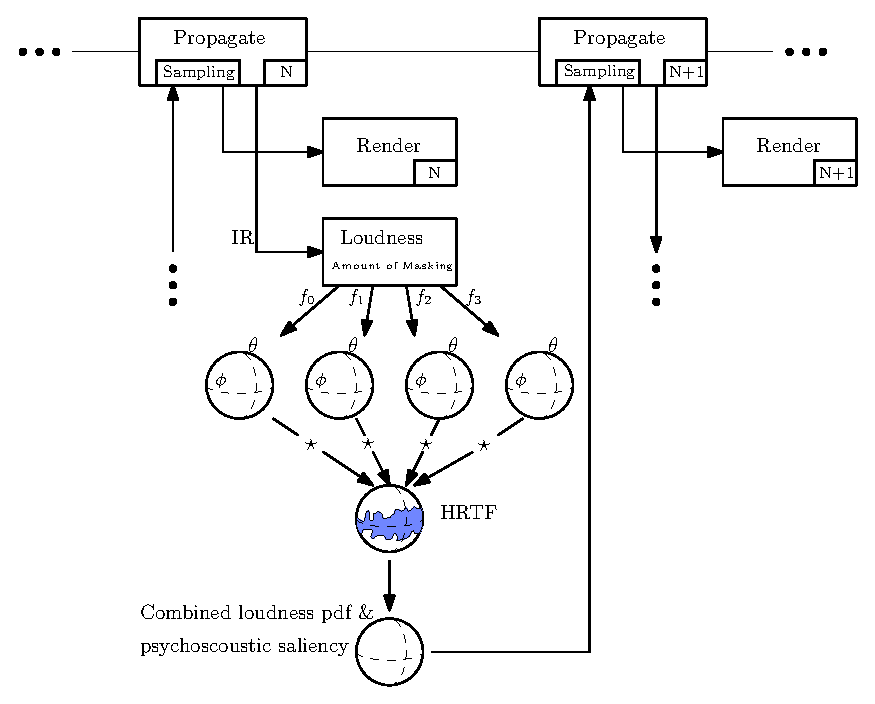
\includegraphics[width=3.0in]{figs/figure1}}
  \caption{Our pipeline}
  \label{fig:figure1}
\end{figure}

The general pipeline of our system consists of a preprocessing step that is performed on source audio
as well as a runtime component that enables feedback from the auralization of IRs computed in one step of 
propagation to accelerate the next step of propagation.
\paragraph{Preprocessing}
Much of the sound processing performed as part of the MPEG Psychoacoustic Model II can be precomputed 
given a clip of audio that will become a source of sound.
We perform a short-time fourier transform of the audio using 512 sample-wide Hanning windows with a 
50\% overlap between neighboring windows.
We store this in an augmented representation of the source's sound buffer that can interpolate between 
windowed spectrograms to arrive at the frequency representation of the audio corresponding to a specific 
path's delay and start time.
Likewise, we also store and interpolate the power spectral density, tonality, and Bark critical bands 
precomputed from this frequency representation.
When the frequency bands that will be used to discretize sound in the impulse response are known, the 
spreading function used in excitation and masking computations as well as the offsets corresponding 
to noise-masking-tone and tone-masking-noise can also be precomputed.
As is also done in the Psychoacoustic Model II and the work of Nikolas et al, we assume a negligable 
effect due to noise-masking-noise and that the global masking threshold is adequately characterized 
by only the former two.
\paragraph{Perceptual Salience}
Given an impulse response corresponding to propagation step $n$ of the simulation, we compute a measure 
of perceptual salience based on the directionality of loudness and the amount of masking between sampled 
paths that are nearby in time and frequency.
We assume temporal locality of the IR and use this measure of salience as prior knowledge to accelerate 
step $n+1$ of the propagation system.
\paragraph{}
%The computation of perceptual salience involves directional functions that we must represent using a 
%spherical mapping onto a grid of values and rasterize discrete samples onto.
%These spherical functions will ultimately be used for the construction of a probability density function
%of the chance a direction will be samp
For each path of an IR from propagation step $n$, we use it's associated delay to retrieve the precomputed tonality
and power spectral density of the source's sound at that time.
We then compute it's excitation pattern by convolving the precomputed spreading function with the path's power 
spectral density and frequency-binned response.
We also compute for each path it's contribution to the masking threshold of hearing by combining the tone-masking-noise and noise-masking-tone models based on tonality of the signal and store this as an array
of frequency binned thresholds sampled in time.
\paragraph{}
We assume the perceptual salience of a direction from the listener is proportional to the excitation from that direction
above the masking threshold.
We therefore compute our measure of salience as the amount of excitation from that direction above 
the corresponding threshold associated with the path's delay.
The salience of each path is then rasterized onto a spherical mapping of a grid representing directions about the 
listener. 
Because we are sampling discrete, possibly sparse, paths onto a spherical function that will ultimately be used as a 
a probability density function, we rasterize the path's salience onto the sphere using a gaussian kernel 
instead of the nearest cell (as is done in kernel density estimation).
\paragraph{Path Sampling}
Paths at propagation step $n+1$ are sampled around the listener by Monte-Carlo sampling of the 
spherical salience function generated from the IR of propagation step $n$.
The probability of sampling a path from a given direction becomes proportional to the normalized 
salience in that direction and the path's sound power is then inversely scaled by the normalized 
salience as a bias correction.
As a result, paths that are perceptually negligible in their contribution to the final rendered audio 
will be sampled less often and fewer paths will be needed to converge to an accurate IR of the scene.
\paragraph{gSound}
In our gSound implementation, we perform the per-sound precomputation as the scene is loaded and combine our 
representation with that of the sound buffers and sources.
This accounts for the bulk of processing, the remainder of which is handled per-IR.
For the runtime component we have inserted our system as a separate IR update job running in the same threadpool
as the main system that is executed for each freshly computed IR.
The current salience measure is used in propagation as the next is computed from the most recent IR and is accessible 
for visualization through the main propagation system.
\paragraph{}
Both the sampled and discrete path IR are used to compute salience, and so potentially numerous samples might be 
rasterized to the sphere as a result.
We therefore perform the kernel density estimation of spherical functions by rasterizing each discrete sample to it's 
nearest cell and performing several box filters to approximate a gaussian kernel as a post-processing step.
This approach is much more efficient than rasterizing individual gaussian functions and produces similar results.
In order to avoid distortion from box filtering the 2d grid directly, our spherical mapping is a per-hemisphere 
Lambert cylindrical projection.
